\scanpage{32}
\uline{Lemme} \unsure{Soient|Soit} $\Gamma,\Gamma'$ deux polygônes \deleted{\unsure{tels que} $\Gamma=$} \inserted{distinct,} alors $\Gamma\not\subset\Gamma'$, $\Gamma'\not\subset\Gamma$, et $\Gamma\cap\Gamma'$ est une réunion finie d'arcs disjoints de $\Gamma$ (ou de $\Gamma'$), éventuellement réduits à un point.
\figure{%
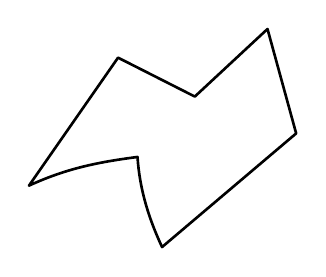
\begin{tikzpicture}[x=.013cm,y=-.013cm,line cap=round,line join=round]
  \draw[line width=.95pt] (274,1178)--(361,1053)--(436,1091)--(507,1025)
    --(535,1127)--(404,1238).. controls (390,1208) and (382,1180) ..(380,1150)
    .. controls (342,1155) and (311,1161) ..(274,1178)--cycle;
\end{tikzpicture}}
Si $\Gamma'=\partial E(\Gamma)$, où $\Gamma$ est un polygône (non convexe puisque $\Gamma'\ne\Gamma$), alors l'\deleted{\unsure{ens}} \inserted{$\Phi$ des} extrémités des arcs polygonaux composantes connexes de $\Gamma\cap\Gamma'$ \deleted{sont des sommets de $\Gamma$} \inserted{est $\subset S(\Gamma)$} alors toute \deleted{telle} $s\in\Phi$, $\exists\,\deleted{\unsure{E}}t\in\Phi$, $t\ne s$, telle que $]s,t[\subset\Gamma'\deleted{\unsure{\operatorname{Ext}}}\cap\complement\Gamma$ et alors $]s,t[\subset\operatorname{Ext}\Gamma$.

% slanted
\margin{\uline{NB} $t$ est unique, sauf si $s$ point isolé de $\Gamma\cap\Gamma'$, auquel cas il existe \unsure{exactmt|exactem} deux tels $t$.}

\uline{Cor} Si $\Gamma$ polygône non convexe, $\exists\,s,s'$ sommets distinct de $\Gamma$, tel que $s$ \deleted{et $s'$, \unsure{visib} de $s$} $]s,s'[\subset\operatorname{Ext}\Gamma\cap\partial E(C)$

[\uline{NB} $\operatorname{Ext}(\Gamma)$ est défini pour tt polygône, pas néc. un 'J-polygône\unsure{.-|..} ]
% archive sheet number: 31
